\documentclass[11pt,wide]{mwart}

\usepackage[utf8]{inputenc}
\usepackage{polski}
\usepackage{graphicx}
\usepackage{hyperref}
\usepackage{amsmath,amssymb,amsfonts,amsthm,mathtools}
\usepackage{float}
\usepackage{enumerate}

\date{Wrocław, \today}
\title{\LARGE\textbf{Pracownia z analizy numerycznej}\\Pracownia P1 Zadanie 12}
\author{Mikołaj Korobczak}

\begin{document}
\maketitle
\begin{center}
Prowadzący: dr hab. Paweł Woźny
\end{center}
\thispagestyle{empty}
\tableofcontents

\section{Wstęp}
Wektor położenia ciała na orbicie eliptycznej w czasie $t$ można liczyć wzorem
\begin{equation}
\Big( a(\cos E - e), a\sqrt[]{1-e^2} \sin E\Big),
\end{equation}
gdzie $a$, to półoś wielka orbity, $e$, to mimośród orbity (ang.eccentricity), natomiast $E$, to anomalia mimośrodowa (ang. eccentric anomaly). Wielkości te obrazuje Rysunek \ref{R1}.
\begin{figure}[H] \label{R1}
	\begin{center}
	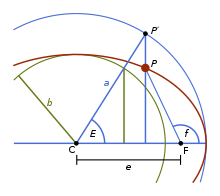
\includegraphics[scale=0.7]{Eccentric_Anomaly}
	\end{center}
	\caption{Szukamy wartości kąta E.}
\end{figure}
Wartości $a$ oraz $e$, to stałe dla każdej planety i nie ma problemu, aby je zdobyć. Wartość $M$ zależy od czasu $t$ przez zależność 
\begin{equation}
M = \frac{2\pi t}{T},
\end{equation}
gdzie $T$, to okres orbitalny planety.
Widać więc, że M nie jest trudno obliczyć. Pozostaje zatem obliczyć wartość kąta $E$. Można go obliczyć z równania Keplera:
\begin{equation}
E - e \sin E = M \qquad (0 < |e| < 1)
\end{equation}
co okazuje się trudnym zadaniem, a do rozwiązania go używa się różnych metod numerycznych. Postanowiłem więc zbadać różne sposoby przybliżenia szukanej wartości, oraz zestawiono wyniki.
Do testów użyte zostały dane z 1 stycznia 2019 roku, a większość przykładów pokazanych jest dla Marsa.

\section{Ograniczenie wartości E}
Aby móc przybliżać wartości metodą bisekcji potrzebujemy odpowiedniego ograniczenia przedziału, w którym znajduje się szukana wartość. Jednym z przybliżeń może być $M - |e| \leq E \leq M + |e|$ dla $0 <|e| < 1$, ale potrzebny jest formalny dowód poprawności takiego przybliżenia. \\
Wiadomo, że $M = x - e \sin x$, gdzie $x = E$, oraz $0 < |e| < 1$
\begin{align*}
M - |e| &\leq x \leq M + |e|\\
x - e \sin x - |e| &\leq x \leq x - e \sin x + |e| \\
-e \sin x -|e| &\leq 0 \leq -e \sin x + |e|\\
-|e| &\leq e \sin x \leq |e|
\end{align*}
\qed \\
% W pierwotnej wersji było takie przybliżenie, ale postanowiłem użyć powyższego zaczerpniętego z artykułu
%Takie przybliżenie jest dobre, ale można się zastanowić czy nie ma lepszego ograniczenia. Innym, lepszym pomysłem może być ograniczenie przez $M \pm |e| \sin x$. 
%\begin{align*}
%M - |e| \sin x &\leq x \leq M + |e| \sin x \\
%x - e \sin x - |e| \sin x &\leq x \leq x - e \sin x + |e| \sin x \\
%- e \sin x - |e| \sin x &\leq 0 \leq -e \sin x + |e| \sin x \\
%- |e| \sin x &\leq e \sin x \leq |e| \sin x \\
%-|e| &\leq e \leq |e|
%\end{align*}
%\qed \\
%Problem z takim ograniczeniem jest taki, że używamy w nim wartości $x$, którą chcemy obliczyć, więc w swoim programie używam pierwszego, ogólniejszego przybliżenia.

Jeszcze dokładniejszym ograniczeniem może być:\footnote{Ograniczenie opisane w G. R. Smith, A simple, efficient starting value for the iterative solution of Kepler’s equation, Celestial Mechanics 19 (1979), 163–166.} \\
Dla $0 \leq M \leq \frac{\pi}{2} - e$
\begin{equation*}
\frac{\frac{\pi}{2}}{\frac{\pi}{2} - e} \leq E \leq M + e
\end{equation*}
Natomiast dla $\frac{\pi}{2} - e \leq M \leq \pi$
\begin{equation*}
\frac{\pi}{\frac{\pi}{2} + e} \Big( \frac{M}{2} + e \Big) \leq E \leq M + e
\end{equation*}
W trakcie wykonwywanych testów używano pierwszego ograniczenia.

\section{Metoda bisekcji} \label{Biskecja}
Jedną z najprostszych metod przybliżania wartości jest metoda bisekcji, która polega na wyznaczeniu przedziału, na którym będziemy szukać miejsca zerowego zadanej funkcji. W badanym przypadku aby oszacować wartość $E$, będziemy szukać w przedziale $\langle M - |e|, M + |e|\rangle$, a naszą funkcją będzie równanie Keplera
\begin{equation}
E - e \sin E - M = 0.
\end{equation}
Bisekcja w każdej iteracji dzieli zadany przedział na pół i szuka miejsca zerowego w jednej z połówek pierwotnego przedziału. Zbieżność tej metody jest liniowa, co widać na naszym przykładzie.  \\
\begin{figure}[H]
	\begin{center}
	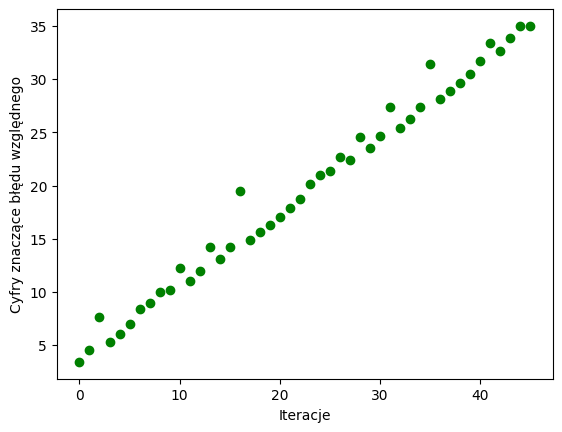
\includegraphics[scale=0.6]{bisekcja}
	\end{center}
	\caption{Zbieżność metody bisekcji.}
\end{figure}
Potrzeba było ponad 40 literacji, aby przybliżenie naszej wartości było dostatecznie dobre.


\section{Metoda iteracyjna} \label{Iteracja}
Inną metodą jest metoda iteracyjna zadana wzorem:
\begin{equation}
x_{n+1} = e \sin(x_n) + M \qquad x_0 = 0.
\end{equation}
Taka metoda wydaje się dobra, ponieważ zwraca od razu przybliżoną wartość $E$, a nie przedział, na którym znajduje się szukana wartość. Nie wymaga zatem, aby pierwsze przyliżenie wartości było dobre (zawsze zaczynamy od wartości 0), a zarazem jest szybciej zbieżna niż metoda bisekcji. Po przetestowaniu tej metody dla takich samych danych, jak w metodzie biskecji, otrzymałem wyniki zobrazowane na wykresie.\\
\begin{figure}[H]
	\begin{center}
	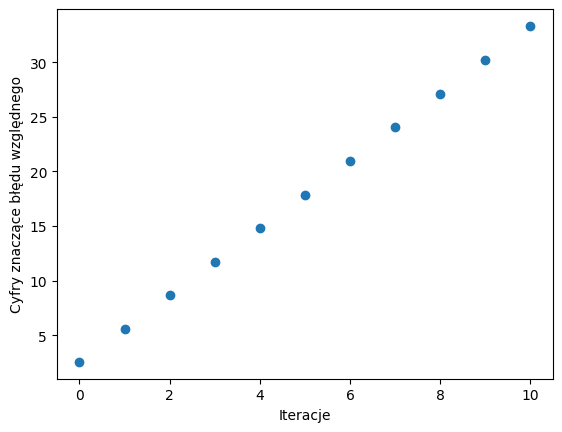
\includegraphics[scale=0.6]{iteracja}
	\end{center}
	\caption{Zbieżność metody iteracyjnej.}
\end{figure}
Niestety metoda ta ma wady, które opisałem w rozdziale \ref{Problemy}.

\section{Metoda Newtona} \label{Newton}
Kolejną metodą przybliżenia poszukiwanej wartości jest metoda Newtona wyrażona wzorem
\begin{equation}
x_{n+1} = x_n - \frac{f(x_n)}{f'(x_n)}.
\end{equation}
Metoda ta jest zbieżna kwadratowo, ale wymaga, aby funkcja wyjściowa była różniczkowalna, ponieważ we wzorze używana jest jej pierwsza pochodna. Ponadto musi ona spełniać kryterium $\forall_{x} f'(x) \ne 0$. Pochodna równania Keplera istnieje i jest wyrażona wzorem
\begin{equation}
f'(x) = 1 - e \cos E \qquad 0 < |e| < 1,
\end{equation}
a ponadto jej wartość nigdy nie wynosi 0. Potrzeba jeszcze startowego przybliżenia wartości x. W tym badaniu użyłem przybliżenia $x_0 = M + \frac{e}{2}$.\footnote{Wartość wybrana w oparciu o artykuł  R. Esmaelzadeh, H. Ghadiri, Appropriate Starter for Solving the Kepler’s Equation, International Journal of Computer Applications 89 (2014), 31–38.} \\
Zbieżność tej metody jest z pewnością lepsza niż poprzednich, co najlepiej obrazuje wykres. \\
\begin{figure}[H]
	\begin{center}
	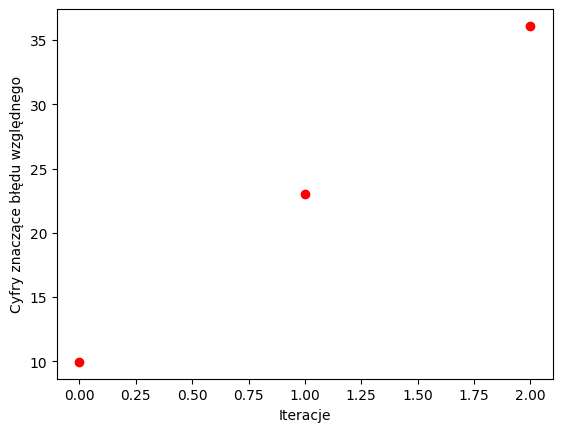
\includegraphics[scale=0.6]{newton}
	\end{center}
	\caption{Zbieżność metody Newtona.}
\end{figure}
\noindent Widać tutaj, że metoda ta wymaga najmniej iteracji, aby osiągnąć wystarczająco dobry wynik.\\

Ostateczne zestawienie zbieżności wszystkich trzech metod pokazuje poniższy wykres.\\
\begin{figure}[H]
	\begin{center}
	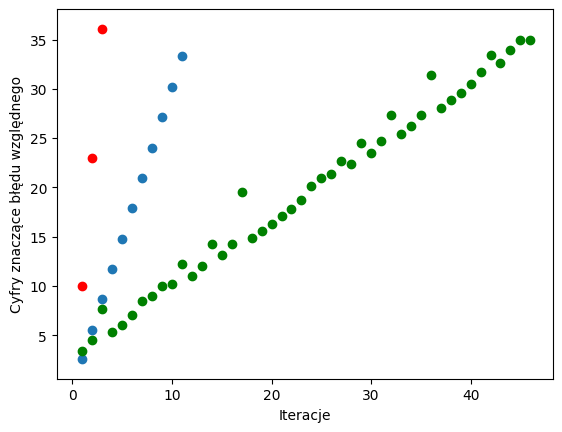
\includegraphics[scale=0.6]{zestawienie_3}
	\end{center}
	\caption{Zestawienie wszystkich metod}
\end{figure}

\section{Inne przykłady}
Aby upewnić się, że wyniki te mają odzwierciedlenie dla innych planet, wykonałem testy dla Merkurego, Wenus i Ziemi. Wykniki zbieżności powyższych metod są podobne, co oznacza, że metody działają w sposób zbliżony dla różnych danych.
\begin{figure}[H]
	\begin{center}
	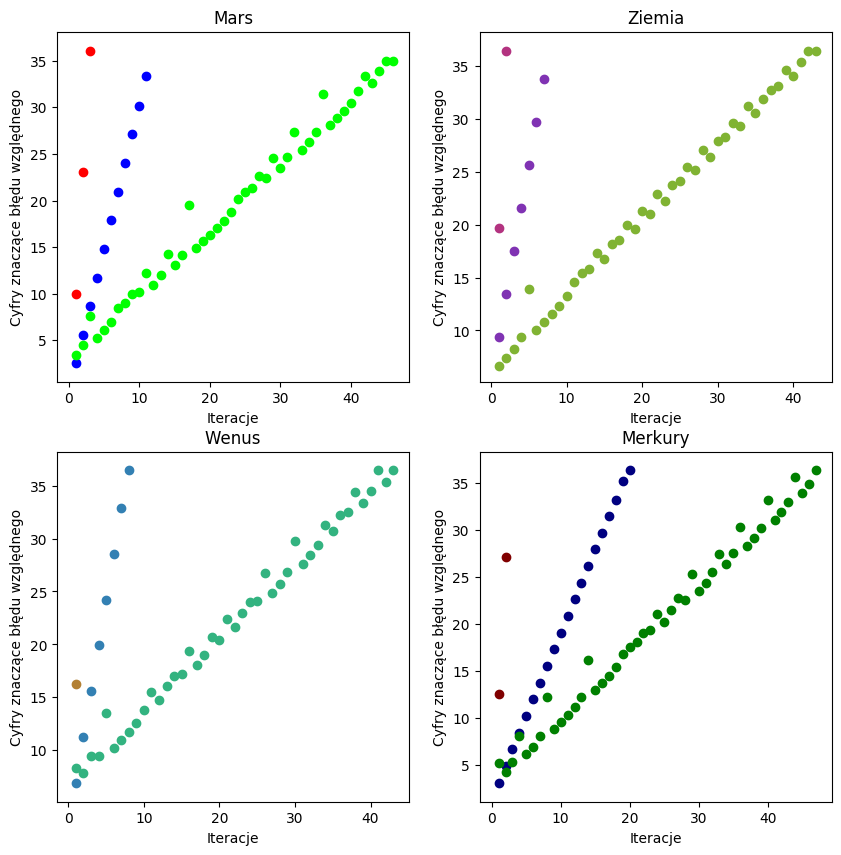
\includegraphics[scale=0.5]{zestawienie_planety}
	\end{center}
	\caption{Inne przykłady.}
\end{figure}
Po przedstawieniu wszystkich tych wyników na wykresie, widać, że metoda bisekcji (odcienie zieleni) jest najwolniej zbieżna, natomiast metoda Newtona (odcienie czerwieni) --- najszybciej.\\
\begin{figure}[H]
	\begin{center}
	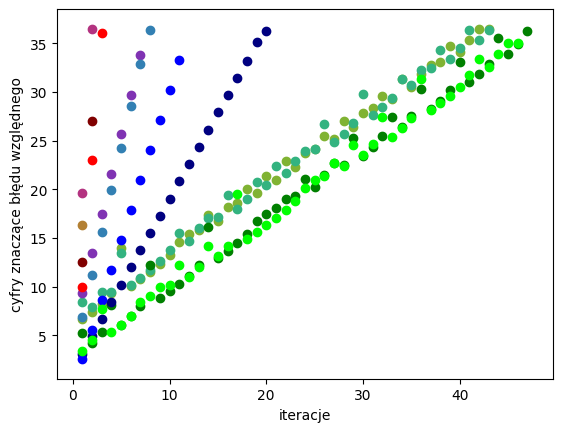
\includegraphics[scale=0.6]{zestawienie_wszystko}
	\end{center}
	\caption{Zestawienie wszystkich testów.}
\end{figure}

\section{Problemy funkcji iteracyjnej} \label{Problemy}
W trakcie badań metody iteracyjnej, opisanej dokładniej w rozdziale \ref{Iteracja}., zauważyłem, że metoda ta czasami zachowuje się nieprzewidywalnie. Jeżeli weźmiemy bardzo dużą wartość mimośrodu orbity $e$, to okazuje się, że funkcja nie zbiega do jednej wartości, co obrazuje poniższy wykres dla $e = 10$.\\
\begin{figure}[H]
	\begin{center}
	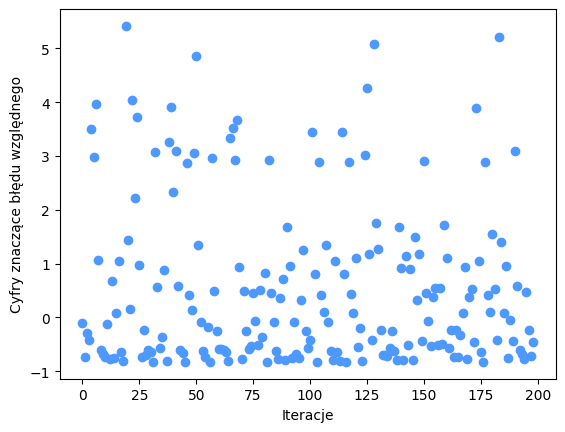
\includegraphics[scale=0.6]{iteracja_rozbieznosc}
	\end{center}
	\caption{Wykres funkcji iteracyjnej dla dużego $e$.}
\end{figure}
Postanowiłem eksperymentalnie sprawdzić na ile utrudnia to poszukiwanie wartości $E$. Poszukałem najmniejszej wartości $e$, dla której funkcja ta nie zbiega i okazało się, że dla  $e \geq 1.302$ tracimy zbieżność\footnote{Wartość szukana z dokładnością $\pm 0.001$}. Jednak kiedy sprawdzimy wartości $e$ dla różnych planet naszego układu słonecznego (Tabela \ref{Tab}), okazuje się, że największa wartość $e$ jest rzędu $10^{-1}$ (dla Merkurego), więc problem ten nie wpływa na wyniki.\\
\begin{table}[H] 

\begin{center}

\begin{tabular}{|c|c|} \hline
Planeta & Mimośród orbity $e$ \\ \hline
Merkury & 2.064529232369614E-01 \\
Wenus	& 1.440912442492587E-02 \\
Ziemia	& 2.436387889126406E-02 \\
Mars	& 9.796953375342891E-02 \\
Jowisz	& 4.993906869363410E-02 \\
Saturn	& 5.453988595722793E-02 \\
Uran	& 4.735756806414718E-02 \\
Neptun	& 8.606944879034762E-03 \\ \hline

\end{tabular}
\end{center}
\caption{Wartości $e$ dla różnych planet.}
\label{Tab}
\end{table}

\section{Wnioski}
Opisane powyżej trzy metody szukania wartości anomalii mimośodowej $E$ zadanej planety posiadają zalety i wady. Metoda bisekcji (Rozdział \ref{Biskecja}) jest łatwa do zaprogramowania i nie wymaga, aby zadana funkcja spełniała złożone założenia (wymaga jedynie, aby funkcja była ciągła na zadanym obszarze). Największą wadą tej metody jest jednak bardzo wolna zbieżność rzędu 40 iteracji w porównaniu do 3 w metodzie Newtona. \\
\indent Durgą metodą jest metoda iteracyjna (Rozdział \ref{Iteracja}), która okazała się znacznie szybsza niż metoda bisekcji. Jednak wzór tej metody odnosi się wyłącznie do rozwiązania równania Keplera i nie można jej stosować w przypadku innych problemów numerycznych. Kolejną wadą tej metody jest to, że nie zawsze jest ona zbieżna, jak pokazano w rozdziale \ref{Problemy}.\\
\indent Ostatnią testowaną metodą jest metoda Newtona (Rozdział \ref{Newton}), która okazała się najszybsza, ze względu na jej kwadratową zbieżność. Metoda ta potrafi zwrócić wartość już po 2 iteracjach (w przypadku Wenus). Jest to znaczna poprawa względem innych metod. Metoda Newtona wymaga jednak, aby zadana funkcja była różniczkowalna i aby jej pochodna zawsze była różna od zera. Poza tym wartość startowa dla tej metody może się okazać trudna do wyznaczenia i trzeba jej szukać eksperymantalnie, a złe dobranie może poskutkować tym, że nie będzie zachodzić zbieżność. Ponadto w opisanym przypadku jedną ze składowych funkcji jest funkcja sinsus, która skądinąd jest trudna do dokładnego liczenia, a w przypadku metody Newtona trzeba dodadkowo liczyć cosinus, co dodatkowo może spotęgować błędy liczenia. Ponieważ jest to zwykła charakterystyka funkcji sinus i cosinus, nie uwzględniałem tych trudnści odrębnie w prowadzonym badaniu. \\
\indent Podsumowując metoda bisekcji wydaje się być najbardziej niezawodna, ale jest wolno zbieżna, metoda iteracyjna sprawdza się bardzo dobrze w omawianym problemie, a jej zbieżność jest zadowalająca, natomiast najszybą metodą jest metoda Newtona, ale używając jej bardzo łatwo można stracić zbieżność.

\newpage
\section*{Literatura i źródła}
\begin{enumerate}[1)]
\item Wszystkie dane pochodzą ze strony: \url{https://ssd.jpl.nasa.gov/horizons.cgi\#top} [4.11.2019]
\item R. Esmaelzadeh, H. Ghadiri, Appropriate Starter for Solving the Kepler’s Equation, International Journal of Computer Applications 89 (2014), 31–38. 
\item G. R. Smith, A simple, efficient starting value for the iterative solution of Kepler’s equation, Celestial Mechanics 19 (1979), 163–166. 
\item \url{https://en.wikipedia.org/wiki/Eccentric_anomaly} [4.11.2019]
\item \url{https://en.wikipedia.org/wiki/Mean_anomaly} [4.11.2019]
\item \url{http://www.stargazing.net/kepler/ellipse.html} [28.10.2019]
\item \url{http://www.jgiesen.de/kepler/kepler.html} [28.10.2019]
\end{enumerate}

\end{document}